\documentclass[conference]{IEEEtran}
\IEEEoverridecommandlockouts

\usepackage{cite}
\usepackage{amsmath,amssymb,amsfonts}
\usepackage{graphicx}
\usepackage{textcomp}
\usepackage{xcolor}
\usepackage{listings}
\usepackage{url}
\usepackage{hyperref}
\usepackage{tikz}
\usetikzlibrary{shapes.geometric, arrows.meta, positioning, fit, backgrounds, calc}
\usepackage{float}
\usepackage{booktabs}
\usepackage{tabularx}

% Code listing style
\lstdefinestyle{codestyle}{
    backgroundcolor=\color{gray!10},
    basicstyle=\ttfamily\scriptsize,
    breaklines=true,
    frame=single,
    numbers=left,
    numberstyle=\tiny\color{gray},
    keywordstyle=\color{blue},
    commentstyle=\color{green!50!black},
    stringstyle=\color{red!70!black},
    showstringspaces=false,
    tabsize=2
}
\lstset{style=codestyle}

\def\BibTeX{{\rm B\kern-.05em{\sc i\kern-.025em b}\kern-.08em
    T\kern-.1667em\lower.7ex\hbox{E}\kern-.125emX}}

\begin{document}

\title{Rasool: A Serverless Cloud-Based Warranty and Product Tracking Application on AWS}

\author{\IEEEauthorblockN{Rasool Basha Durbesula}
\IEEEauthorblockA{Student ID: x24205478 \\
MSc in Cloud Computing \\
National College of Ireland, Dublin \\
x24205478@student.ncirl.ie}}

\maketitle

% ============================================================
% ABSTRACT
% ============================================================
\begin{abstract}
This paper presents the design, implementation, and deployment of Rasool, a cloud-native warranty and product tracking application built entirely on Amazon Web Services using a serverless architecture. The application enables users to register products, manage warranty information, upload supporting documents, track service history, and receive automated reminders for expiring warranties. The system employs six AWS cloud services programmatically, namely AWS Lambda, Amazon DynamoDB, Amazon S3, Amazon API Gateway, Amazon Cognito, and Amazon CloudWatch, each selected after critical evaluation of alternatives. A custom Python library named \texttt{warranty-tracker-nci} was developed and published to the Python Package Index to encapsulate core business logic including warranty status calculation, product validation, document processing, and reminder generation. The frontend is a single-page application built with React and Tailwind CSS, hosted on Amazon S3 as a static website. A continuous integration and deployment pipeline implemented through GitHub Actions automates library testing, backend deployment via the Serverless Framework, and frontend distribution to S3. The application is publicly accessible and demonstrates the practical application of cloud architectural patterns such as the serverless compute pattern, event-driven architecture, and the API gateway pattern. This report critically analyses the architectural decisions, documents the implementation of all CRUD operations and cloud service integrations, and reflects on the challenges and learnings encountered during development.
\end{abstract}

\begin{IEEEkeywords}
Serverless Architecture, AWS Lambda, DynamoDB, Cloud Computing, Warranty Management, CI/CD, Python Library, React
\end{IEEEkeywords}

% ============================================================
% I. INTRODUCTION
% ============================================================
\section{Introduction}

Managing product warranties is a common challenge faced by consumers and businesses alike. Warranty documents are frequently misplaced, expiry dates are forgotten, and service records are scattered across various formats and locations. As cloud computing has matured, serverless architectures have emerged as a compelling paradigm for building scalable, cost-effective applications without the overhead of server management \cite{jonas2019cloud}. This project leverages the serverless computing model to address the warranty management problem through a fully cloud-native application.

The primary motivation behind Rasool is to provide a centralised, accessible, and automated solution for warranty tracking. The application allows authenticated users to register their products, attach warranty details with supporting documents, log service history, and receive proactive notifications when warranties approach their expiration dates. By deploying entirely on AWS, the application takes advantage of managed services that offer automatic scaling, high availability, and a pay-per-use billing model \cite{awswell2023}.

The main objectives of this project are as follows. First, to design and implement a cloud-based application that employs at least five AWS services programmatically. Second, to develop a reusable Python library that encapsulates core business logic independent of the cloud provider. Third, to implement full CRUD operations across multiple data entities. Fourth, to establish a CI/CD pipeline that automates testing and deployment. Fifth, to deploy the application on a public cloud platform and make it accessible via a public URL.

This report documents the full lifecycle of the project from requirements specification through architecture design, implementation, deployment, and reflection. The subsequent sections are organised as follows: Section II presents the project specification and requirements, Section III discusses the architecture and design, Section IV describes the custom library, Section V analyses the cloud services used, Section VI details the implementation, Section VII covers continuous integration and deployment, and Section VIII concludes with findings and reflections.

% ============================================================
% II. PROJECT SPECIFICATION AND REQUIREMENTS
% ============================================================
\section{Project Specification and Requirements}

\subsection{Functional Requirements}

The application supports four core data entities: Products, Warranties, Service History, and Documents. For each of the first three entities, full CRUD (Create, Read, Update, Delete) operations are provided through RESTful API endpoints secured with JWT-based authentication. The API follows a consistent design pattern where each entity has five endpoints corresponding to the create, list, get, update, and delete operations, all routed through Amazon API Gateway and protected by a Cognito User Pool authoriser.

The product management module allows users to register products with attributes including name, brand, category, model number, serial number, purchase date, purchase price, and retailer. The system validates incoming product data against a predefined set of categories (Electronics, Appliances, Furniture, Automotive, Sports and Outdoors, Tools, Clothing, and Other) and ensures that required fields such as name, brand, category, and purchase date are present before persisting the record to DynamoDB. The warranty management module links warranties to registered products through a \texttt{product\_id} foreign key relationship and supports fields such as provider, start date, end date, warranty type, and coverage details. Warranty responses are enriched server-side with computed fields including a status classification (active for more than thirty days remaining, expiring for thirty days or fewer, or expired for past the end date) and the exact number of days remaining until expiry. This server-side enrichment ensures that all clients receive consistent status information without duplicating date-calculation logic.

The service history module enables users to log maintenance, repair, inspection, and replacement records against registered products, with each record capturing the service date, type, description, provider, and associated cost. The service history listing endpoint supports an optional \texttt{product\_id} query parameter, allowing the frontend to display service records contextualised to a specific product. The document management module generates presigned S3 URLs for secure, direct file uploads and downloads without exposing AWS credentials to the client. Supported file types include PDF, JPEG, PNG, and Word documents, with a maximum file size of ten megabytes enforced by the custom library's validation logic.

An automated reminder system, triggered daily through CloudWatch Events using a scheduled cron expression, scans all warranties across all users and identifies those expiring within thirty days. For each expiring warranty, the system generates a structured notification payload containing the product name, warranty provider, end date, and days remaining. User authentication is handled through Amazon Cognito, which manages user registration with email verification, secure login using the Secure Remote Password protocol, and JWT token issuance for stateless API authentication.

\subsection{Non-Functional Requirements}

The application must be scalable to handle varying user loads without manual intervention, which is achieved through the inherent auto-scaling capabilities of serverless services. Each AWS Lambda function scales independently in response to incoming requests, and DynamoDB's on-demand capacity mode adjusts read and write throughput automatically based on actual traffic patterns. Security is enforced at multiple layers following a defence-in-depth strategy: API Gateway validates Cognito JWT tokens before invoking Lambda functions, each Lambda handler extracts the authenticated user's \texttt{sub} claim from the JWT and uses it to scope all DynamoDB queries, ensuring strict data isolation between users, and S3 document access is controlled through time-limited presigned URLs that expire after one hour. The application must maintain low latency for API responses, supported by DynamoDB's single-digit millisecond performance for key-value operations and Lambda's lightweight execution model with a configured timeout of thirty seconds \cite{sbarski2017serverless}. Cost efficiency is a key priority for this project, and the combination of DynamoDB's on-demand billing (charged per read and write request unit), Lambda's per-invocation pricing at fractions of a cent, and S3's per-gigabyte storage cost ensures that the total operational expense scales linearly with actual usage rather than requiring upfront capacity commitments. The frontend must be responsive and accessible across desktop and mobile devices, which is achieved through Tailwind CSS's utility-first responsive design framework combined with React's component-based architecture. Reliability is addressed through the inherent redundancy of AWS managed services, where Lambda functions execute across multiple Availability Zones and DynamoDB automatically replicates data across three facilities within the selected region.

% ============================================================
% III. ARCHITECTURE AND DESIGN
% ============================================================
\section{Architecture and Design}

The application follows a three-tier serverless architecture comprising a static frontend tier, a serverless API tier, and a managed data tier. This architectural approach aligns with the AWS Well-Architected Framework's serverless application lens, which advocates for the use of managed services to reduce operational complexity and improve reliability \cite{awswell2023}.

\subsection{Architecture Diagram}

Figure~\ref{fig:architecture} presents the complete architecture of the Rasool application, illustrating the interaction between all six AWS cloud services and the client-side application.

\begin{figure*}[!ht]
\centering
\resizebox{\textwidth}{!}{%
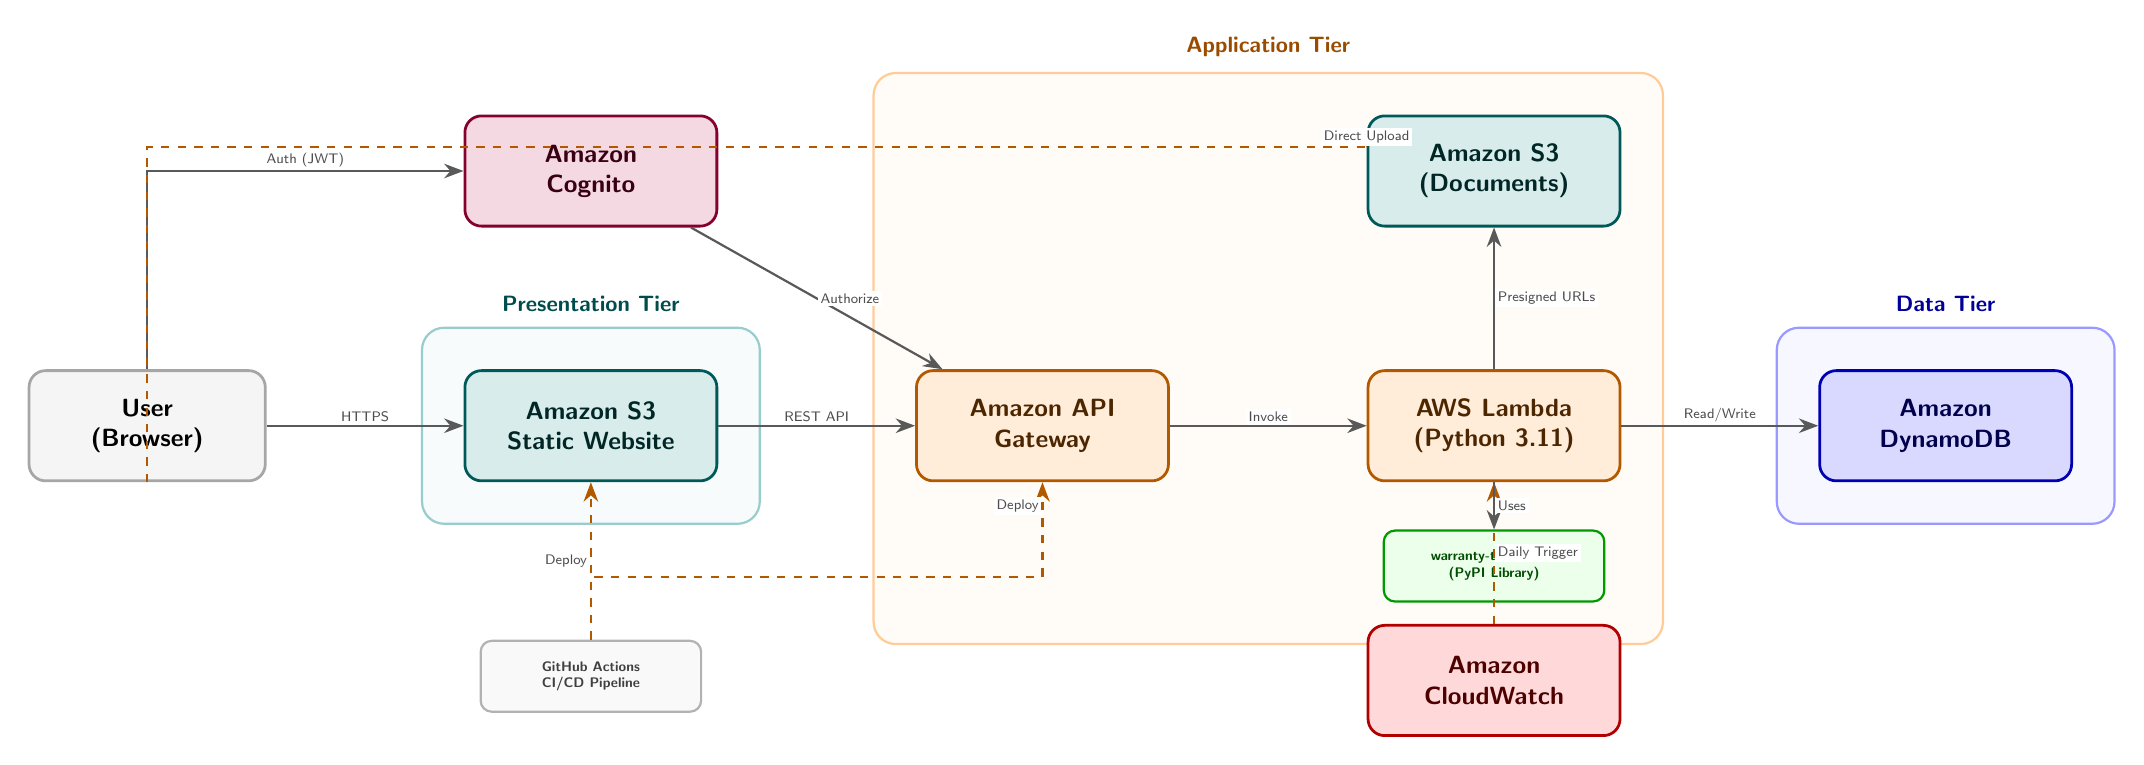
\begin{tikzpicture}[
    node distance=1.5cm and 2.2cm,
    every node/.style={font=\sffamily\small},
    service/.style={rectangle, rounded corners=6pt, draw=#1!70!black, fill=#1!15,
        minimum width=3.2cm, minimum height=1.4cm, align=center, line width=1pt,
        text=#1!30!black, font=\sffamily\small\bfseries},
    service/.default=blue,
    userbox/.style={rectangle, rounded corners=6pt, draw=gray!70, fill=gray!8,
        minimum width=3cm, minimum height=1.4cm, align=center, line width=1pt,
        font=\sffamily\small\bfseries},
    arrow/.style={-{Stealth[length=7pt]}, thick, color=gray!70!black},
    dasharrow/.style={-{Stealth[length=7pt]}, thick, dashed, color=orange!70!black},
    label/.style={font=\sffamily\tiny, text=gray!60!black, midway, fill=white, inner sep=1pt},
    tierbox/.style={rectangle, rounded corners=8pt, draw=#1!40, fill=#1!3,
        inner sep=12pt, line width=0.8pt},
    tierbox/.default=blue,
    tierlabel/.style={font=\sffamily\footnotesize\bfseries, text=#1!60!black},
    tierlabel/.default=blue,
]

% --- User ---
\node[userbox] (user) {User\\(Browser)};

% --- Frontend Tier ---
\node[service=teal, right=2.5cm of user] (s3front) {Amazon S3\\Static Website};

% --- Auth ---
\node[service=purple, above=1.8cm of s3front] (cognito) {Amazon\\Cognito};

% --- API Tier ---
\node[service=orange, right=2.5cm of s3front] (apigw) {Amazon API\\Gateway};

% --- Compute ---
\node[service=orange, right=2.5cm of apigw] (lambda) {AWS Lambda\\(Python 3.11)};

% --- Data Tier ---
\node[service=blue, right=2.5cm of lambda] (dynamo) {Amazon\\DynamoDB};
\node[service=teal, above=1.8cm of lambda] (s3docs) {Amazon S3\\(Documents)};
\node[service=red, below=1.8cm of lambda] (cloudwatch) {Amazon\\CloudWatch};

% --- Library ---
\node[rectangle, rounded corners=4pt, draw=green!60!black, fill=green!8,
    minimum width=2.8cm, minimum height=0.9cm, align=center, line width=0.8pt,
    font=\sffamily\tiny\bfseries, text=green!30!black, below=0.6cm of lambda] (lib) {warranty-tracker-nci\\(PyPI Library)};

% --- CI/CD ---
\node[rectangle, rounded corners=4pt, draw=gray!60, fill=gray!5,
    minimum width=2.8cm, minimum height=0.9cm, align=center, line width=0.8pt,
    font=\sffamily\tiny\bfseries, text=gray!50!black, below=2cm of s3front] (cicd) {GitHub Actions\\CI/CD Pipeline};

% --- Tier backgrounds ---
\begin{scope}[on background layer]
    \node[tierbox=teal, fit=(s3front), inner sep=15pt] (fronttier) {};
    \node[tierbox=orange, fit=(apigw)(lambda)(s3docs)(lib), inner sep=15pt] (apitier) {};
    \node[tierbox=blue, fit=(dynamo), inner sep=15pt] (datatier) {};
\end{scope}

% --- Tier labels ---
\node[tierlabel=teal, above=2pt of fronttier.north] {Presentation Tier};
\node[tierlabel=orange, above=2pt of apitier.north] {Application Tier};
\node[tierlabel=blue, above=2pt of datatier.north] {Data Tier};

% --- Arrows ---
\draw[arrow] (user) -- (s3front) node[label, above] {HTTPS};
\draw[arrow] (user) |- (cognito) node[label, near end, above] {Auth (JWT)};
\draw[arrow] (s3front) -- (apigw) node[label, above] {REST API};
\draw[arrow] (apigw) -- (lambda) node[label, above] {Invoke};
\draw[arrow] (lambda) -- (dynamo) node[label, above] {Read/Write};
\draw[arrow] (lambda) -- (s3docs) node[label, right] {Presigned URLs};
\draw[arrow] (cognito) -- (apigw) node[label, right] {Authorize};
\draw[dasharrow] (cloudwatch) -- (lambda) node[label, right] {Daily Trigger};
\draw[arrow] (lambda) -- (lib) node[label, right] {Uses};
\draw[dasharrow] (cicd) -- (s3front) node[label, left] {Deploy};
\draw[dasharrow] (cicd) |- ([yshift=-1.2cm]apigw.south) -- (apigw) node[label, left, near end] {Deploy};
\draw[dasharrow] (user.south) |- ([yshift=0.3cm]s3docs.west) -- (s3docs) node[label, above, near end] {Direct Upload};

\end{tikzpicture}
}%
\caption{Architecture diagram of the Rasool warranty tracking application showing the interaction between six AWS services, the custom PyPI library, and the CI/CD pipeline.}
\label{fig:architecture}
\end{figure*}

\subsection{Architectural Patterns}

The application employs several well-established cloud architectural patterns. The \textit{serverless compute pattern} eliminates server provisioning and management by delegating all backend logic to AWS Lambda functions, which execute on demand and scale automatically in response to incoming requests \cite{jonas2019cloud}. The \textit{API gateway pattern} provides a single entry point for all client requests, handling routing, authentication validation, and CORS enforcement before forwarding requests to the appropriate Lambda function \cite{richardson2018microservices}. The \textit{event-driven pattern} is utilised for the warranty reminder system, where CloudWatch Events triggers a Lambda function on a daily schedule to scan for expiring warranties. The \textit{static content hosting pattern} serves the React single-page application from an S3 bucket configured for static website hosting, eliminating the need for a web server. The \textit{Backend for Frontend (BFF) pattern} is implicitly applied as the API layer is designed specifically to serve the frontend's data requirements, with warranty responses enriched server-side to include computed status fields.

\subsection{Critical Analysis of Design Decisions}

The choice of a serverless architecture over a containerised approach using Amazon ECS or EKS was driven by the application's request-driven nature and the desire to minimise operational overhead. While containers offer greater runtime flexibility, Lambda's automatic scaling and per-invocation billing model better suit an application with variable and potentially low traffic patterns \cite{sbarski2017serverless}. However, this design introduces cold start latency, which can affect the responsiveness of infrequently invoked functions. To mitigate this, the Lambda functions are configured with a modest 256MB memory allocation, which also influences CPU allocation and reduces cold start duration.

The decision to use DynamoDB over Amazon RDS was informed by the application's data access patterns, which primarily involve key-value lookups and queries on Global Secondary Indexes. DynamoDB's schemaless design accommodates the varying attributes of products, warranties, and service records without requiring schema migrations. The trade-off is the lack of support for complex relational queries, which is acceptable given that the application does not require cross-entity joins.

% ============================================================
% IV. LIBRARY DESCRIPTION
% ============================================================
\section{Library Description}

A custom Python library named \texttt{warranty-tracker-nci} was developed to encapsulate the core business logic of the application. The library is published on the Python Package Index (PyPI) and is available at \url{https://pypi.org/project/warranty-tracker-nci/}. The rationale behind creating this library was to separate domain-specific logic from cloud infrastructure concerns, enabling reusability across different deployment contexts and facilitating unit testing without requiring AWS service mocks.

The library comprises four primary modules. The \texttt{WarrantyManager} class handles warranty data validation, status calculation, and warranty enrichment. It validates that all required fields are present and that dates conform to the ISO 8601 format, computes whether a warranty is active, expiring (within thirty days), or expired, and enriches warranty records with computed status and days-remaining fields. The \texttt{ProductManager} class provides product data validation against a predefined set of categories including Electronics, Appliances, Furniture, and Automotive, and offers a keyword-based category suggestion feature. The \texttt{DocumentProcessor} class validates file types against an allowlist (PDF, JPG, PNG, DOC, DOCX), enforces a ten-megabyte size limit, generates structured S3 keys, and extracts document metadata including MIME content types. The \texttt{ReminderScheduler} class filters expiring warranties and generates structured email notification payloads.

The library is integrated into the Lambda backend through direct imports. The following code snippet demonstrates how the \texttt{WarrantyManager} is used in the warranties handler to enrich API responses:

\begin{lstlisting}[language=Python, caption={Usage of WarrantyManager in Lambda handler}]
from warranty_tracker import WarrantyManager

manager = WarrantyManager()

def list(event, context):
    user_id = get_user_id(event)
    warranties = query_by_index(
        WARRANTIES_TABLE, 'user_id-index',
        'user_id', user_id)
    enriched = [manager.enrich_warranty(w)
                for w in warranties]
    return success(enriched)
\end{lstlisting}

The \texttt{enrich\_warranty} method adds the \texttt{status} and \texttt{days\_remaining} fields to each warranty record, enabling the frontend to render colour-coded status indicators without performing date calculations on the client side. The library is installed as a dependency during the CI/CD pipeline before the Lambda functions are packaged for deployment, ensuring that the latest version is always included.

% ============================================================
% V. CLOUD SERVICES ANALYSIS
% ============================================================
\section{Cloud-Based Services Analysis}

The application employs six AWS cloud services, each selected after evaluating alternatives and considering factors such as scalability, cost, integration complexity, and alignment with the serverless architecture. Table~\ref{tab:services} provides a summary of each service, its role in the application, and the alternative that was considered during the design phase.

\begin{table}[ht]
\centering
\caption{Summary of AWS Services Used in the Application}
\label{tab:services}
\scriptsize
\begin{tabularx}{\columnwidth}{l X l}
\toprule
\textbf{Service} & \textbf{Role in Application} & \textbf{Alternative} \\
\midrule
Lambda & Serverless compute for API handlers & EC2 / ECS \\
DynamoDB & NoSQL data storage (3 tables) & RDS (PostgreSQL) \\
S3 & Frontend hosting \& document storage & CloudFront / EFS \\
API Gateway & REST API routing \& auth & ALB \\
Cognito & User authentication \& JWT & Custom auth \\
CloudWatch & Logging \& scheduled triggers & EventBridge \\
\bottomrule
\end{tabularx}
\end{table}

\subsection{AWS Lambda}

AWS Lambda serves as the compute layer, executing thirteen Python 3.11 functions that handle all API logic. Lambda was chosen over Amazon EC2 or ECS because the application's workload is event-driven and does not require persistent compute resources. Lambda's automatic scaling ensures that each API request is handled by a dedicated execution environment, and the pay-per-invocation pricing model (currently \$0.20 per million requests) makes it cost-effective for applications with variable traffic \cite{awslambda2024}. The trade-off is a maximum execution duration of fifteen minutes and potential cold start latency, neither of which presents a practical issue for this application's sub-second API operations.

\subsection{Amazon DynamoDB}

DynamoDB provides the NoSQL data layer through three tables: Products, Warranties, and Service History. Each table uses a string-typed partition key (\texttt{id}) populated with UUID version 4 values to ensure uniform distribution across partitions. Global Secondary Indexes (GSIs) are defined on \texttt{user\_id} for all three tables, enabling efficient retrieval of all records belonging to a specific authenticated user. The Warranties and Service History tables additionally define a \texttt{product\_id} GSI, supporting queries that retrieve all warranties or service records associated with a particular product. DynamoDB was selected over Amazon RDS because the application's data access patterns are primarily key-value lookups and GSI queries that do not require relational joins, which DynamoDB serves with consistent single-digit millisecond latency regardless of table size \cite{decandia2007dynamo}. The on-demand (PAY\_PER\_REQUEST) capacity mode eliminates the need to estimate and provision read and write capacity units, automatically scaling throughput from zero to thousands of requests per second in response to traffic patterns without any capacity planning.

\subsection{Amazon S3}

Amazon S3 serves a dual purpose in the application. First, it hosts the React frontend as a static website, configured with an index document and error document for client-side routing. Second, a separate S3 bucket stores warranty documents (PDFs, images, and Word files) uploaded by users. Document uploads and downloads are facilitated through presigned URLs generated by Lambda functions, which grant time-limited access without exposing AWS credentials. S3 was chosen for document storage over Amazon EFS due to its native HTTP accessibility, virtually unlimited storage capacity, and eleven nines of durability \cite{awss3docs}.

\subsection{Amazon API Gateway}

API Gateway provides the RESTful interface between the frontend and Lambda functions. It handles request routing to the appropriate Lambda function, enforces CORS policies for cross-origin browser requests, and validates Cognito JWT tokens through a built-in authoriser before allowing access to protected endpoints. API Gateway was preferred over an Application Load Balancer because it integrates natively with Lambda and Cognito, supports request throttling, and requires no infrastructure management \cite{richardson2018microservices}.

\subsection{Amazon Cognito}

Cognito manages user authentication, providing user registration, email verification, and secure login with JWT token issuance. The frontend uses the \texttt{amazon-cognito-identity-js} SDK to interact with the Cognito User Pool directly, obtaining ID tokens that are subsequently included in API requests. Cognito was chosen over implementing a custom authentication system using bcrypt and JWTs stored in DynamoDB because it provides industry-standard security practices, including password hashing with SRP protocol, token refresh mechanisms, and compliance with OAuth 2.0 standards \cite{awscognito2024}. The User Pool is configured to require a minimum password length of eight characters with uppercase, lowercase, and numeric character requirements.

\subsection{Amazon CloudWatch}

CloudWatch serves two functions in the application. It provides centralised logging for all Lambda function executions, capturing request and error logs for monitoring and debugging. Additionally, CloudWatch Events (EventBridge) triggers the warranty expiry check Lambda function on a daily schedule using a cron expression. This event-driven approach was chosen over a polling mechanism because it is more resource-efficient, executes precisely on schedule, and incurs no cost when the function is not running \cite{awscloudwatch2024}.

% ============================================================
% VI. IMPLEMENTATION
% ============================================================
\section{Implementation}

The implementation comprises a Python 3.11 backend deployed as thirteen AWS Lambda functions, a React 18 single-page application frontend, and the custom \texttt{warranty-tracker-nci} Python library. All CRUD operations are implemented across three data entities (Products, Warranties, and Service History), and the source code includes inline comments explaining the logic and rationale behind key decisions.

\subsection{Backend Implementation}

The backend follows a modular architecture with five handler modules (products, warranties, service history, documents, and reminders) and three utility modules for database operations, authentication token extraction, and standardised API responses. Each handler function begins by extracting the authenticated user's identifier from the Cognito JWT claims using the \texttt{get\_user\_id} utility, which reads the \texttt{sub} claim from the \texttt{requestContext.authorizer.claims} object in the API Gateway event. This ensures that all subsequent DynamoDB queries are scoped to the authenticated user, preventing unauthorised access to other users' data. The database utility module abstracts DynamoDB operations including \texttt{put\_item}, \texttt{get\_item}, \texttt{update\_item}, \texttt{delete\_item}, \texttt{query\_by\_index}, and \texttt{scan\_table}, providing a consistent interface across all handlers and centralising error handling. The response utility module standardises all API responses with appropriate HTTP status codes, CORS headers (Access-Control-Allow-Origin, Access-Control-Allow-Credentials), and a custom \texttt{DecimalEncoder} that serialises DynamoDB's Decimal types to JSON-compatible numbers.

The warranty creation handler demonstrates the integration of the custom library with DynamoDB:

\begin{lstlisting}[language=Python, caption={Warranty creation with library validation}]
from warranty_tracker import WarrantyManager

manager = WarrantyManager()

def create(event, context):
    user_id = get_user_id(event)
    body = parse_body(event)
    # Validate using library
    is_valid, msg = manager.validate_warranty_data(body)
    if not is_valid:
        return error(msg)
    warranty = {
        'id': str(uuid.uuid4()),
        'user_id': user_id,
        **body,
        'created_at': datetime.utcnow().isoformat()
    }
    put_item(WARRANTIES_TABLE, warranty)
    return success(warranty, 201)
\end{lstlisting}

The document handler generates presigned S3 URLs for secure file operations, representing a critical integration point between the frontend, Lambda, and S3. When a user uploads a warranty document, the frontend first sends a POST request to the \texttt{/documents/upload-url} endpoint with the filename, content type, and associated warranty identifier. The Lambda function validates the request, generates a structured S3 key using the pattern \texttt{documents/\{user\_id\}/\{warranty\_id\}/\{uuid\}.\{ext\}}, and calls the S3 client's \texttt{generate\_presigned\_url} method with a one-hour expiration. The frontend then performs a direct PUT request to the returned presigned URL, uploading the file straight to S3 without routing binary data through API Gateway or Lambda. This approach bypasses API Gateway's ten-megabyte payload limitation and significantly reduces backend compute costs and latency for file operations.

\begin{lstlisting}[language=Python, caption={Presigned URL generation for document uploads}]
def get_upload_url(event, context):
    user_id = get_user_id(event)
    body = parse_body(event)
    key = DocumentProcessor.generate_s3_key(
        user_id, body['warranty_id'],
        body['filename'])
    url = s3.generate_presigned_url(
        'put_object',
        Params={'Bucket': BUCKET,
                'Key': key,
                'ContentType': body['content_type']},
        ExpiresIn=3600)
    return success({'upload_url': url, 'key': key})
\end{lstlisting}

The update operations across all entities utilise DynamoDB's \texttt{UpdateExpression} syntax to perform partial updates, modifying only the fields included in the request body rather than replacing the entire item. This approach preserves any fields not included in the update request and reduces the amount of data written to the database. Each update operation also appends an \texttt{updated\_at} timestamp to maintain an audit trail of modifications.

\subsection{Frontend Implementation}

The frontend is a single-page application built with React 18, styled with Tailwind CSS, and bundled using Vite for fast development and optimised production builds. It uses React Router v6 for declarative client-side navigation and Axios for HTTP communication with the backend API, with a request interceptor that automatically attaches the Cognito JWT ID token to the Authorization header of every outgoing request. An \texttt{AuthContext} provider implemented using React's Context API wraps the entire application, managing user session state and exposing \texttt{login}, \texttt{logout}, \texttt{getIdToken}, and \texttt{getUserAttributes} functions to all child components through the \texttt{useAuth} custom hook. A \texttt{ProtectedRoute} component guards authenticated pages by checking the current user state and redirecting unauthenticated visitors to the login page.

The application comprises eleven page components and five reusable UI components. The dashboard page aggregates product and warranty data to display summary statistics including total products, active warranties, expiring warranties, and expired warranties, along with a list of the five most urgently expiring warranties for quick reference. The product management pages include a listing view with search and filter capabilities, a detailed product view showing associated warranties and service history, and forms for adding and editing products with client-side validation. The warranties listing page renders colour-coded status indicators (green for active, yellow for expiring, red for expired) based on the enriched status field returned by the API, and supports filtering by status category. A dedicated \texttt{FileUpload} component provides drag-and-drop file upload functionality with client-side file type and size validation, progress feedback, and toast notifications using the \texttt{react-hot-toast} library. The reminders page groups warranties by status and sorts them by days remaining in ascending order, providing users with an actionable overview of upcoming expirations and enabling them to take timely action before warranty coverage lapses.

% ============================================================
% VII. CI/CD
% ============================================================
\section{Continuous Integration, Delivery and Deployment}

The application employs a fully automated CI/CD pipeline implemented through GitHub Actions, triggered on every push to the main branch of the private GitHub repository. The pipeline consists of three sequential jobs that ensure code quality before deployment.

The first job, \texttt{test-library}, checks out the repository, installs the custom library in editable mode, and executes the test suite using pytest. The test suite covers all four library modules, validating warranty status calculation, product data validation, document processing, and reminder generation. Only when all tests pass does the pipeline proceed to the deployment stages.

The second job, \texttt{deploy-backend}, depends on the successful completion of the test job. It configures AWS credentials from repository secrets, installs the custom library, and deploys the backend using the Serverless Framework. The Serverless Framework packages the Lambda functions with their dependencies and creates or updates the CloudFormation stack that provisions all backend resources including Lambda functions, API Gateway endpoints, DynamoDB tables, S3 buckets, and Cognito User Pools.

The third job, \texttt{deploy-frontend}, depends on the backend deployment completing successfully to ensure that any API changes are live before the frontend is updated. It installs Node.js 18 dependencies, builds the React application using Vite with production environment variables (API URL, Cognito User Pool ID, and Client ID) injected at build time from GitHub repository secrets, and synchronises the compiled static assets to the S3 frontend bucket using the \texttt{aws s3 sync} command with the \texttt{--delete} flag to remove stale files from previous deployments. This sequential dependency chain (test, then backend, then frontend) ensures that a broken library never reaches production and that the frontend always targets a compatible API version.

This pipeline embodies the principles of continuous integration by running automated tests on every code change, continuous delivery by automating the build and packaging process, and continuous deployment by automatically releasing changes to the production environment without manual intervention \cite{awswell2023}. All sensitive configuration values including AWS credentials, API endpoints, and Cognito identifiers are stored as encrypted GitHub Secrets and never exposed in the repository or build logs.

The deployed application is accessible at the following URL: \url{http://warranty-tracker-frontend-prod.s3-website-eu-west-1.amazonaws.com}. The backend API is available at \url{https://yh3dejnvxe.execute-api.eu-west-1.amazonaws.com/prod}. The source code is maintained in a private GitHub repository at \url{https://github.com/Rasool1817/CPP}.

% ============================================================
% VIII. CONCLUSIONS
% ============================================================
\section{Conclusions}

This project successfully demonstrates the design, implementation, and deployment of a complex cloud-based application using six AWS services in a fully serverless architecture. The warranty tracking application provides comprehensive CRUD functionality across products, warranties, service history, and documents, with automated warranty expiry monitoring through event-driven scheduled functions.

Several key findings emerged from this development process. First, the serverless architecture significantly reduced operational complexity by eliminating the need for server provisioning, patching, and capacity planning. The pay-per-use pricing model proved highly cost-effective for a project with variable and modest traffic levels. Second, the decision to develop a custom Python library and publish it to PyPI fostered better separation of concerns, as the business logic could be unit-tested independently of AWS services and could potentially be reused in other contexts. Third, the Serverless Framework proved invaluable for infrastructure-as-code management, enabling reproducible deployments and simplifying the management of interconnected cloud resources.

However, several limitations were identified during development and testing. The application currently logs warranty expiry warnings to CloudWatch rather than sending actual email notifications to users, as the Amazon Simple Email Service (SES) integration was removed due to the email verification requirements imposed by SES sandbox mode, which restricts sending to verified email addresses only. Moving to SES production mode would require submitting a request to AWS with a justification for sending email, which was beyond the scope of this project's timeline. The frontend is served over HTTP from the S3 static website endpoint rather than HTTPS, which represents a security limitation for a production application. Implementing HTTPS would require the addition of Amazon CloudFront as a content delivery network with an SSL/TLS certificate provisioned through AWS Certificate Manager. Furthermore, the application does not implement server-side pagination for list endpoints, relying instead on DynamoDB's default one-megabyte response limit, which could become a performance and cost concern as the number of records per user grows into the thousands. The DynamoDB table design uses a simple partition key rather than a composite key, which means that certain access patterns such as querying warranties by date range require full index scans rather than efficient range queries.

The development process itself presented learning opportunities regarding the intricacies of configuring cross-service integrations within the AWS ecosystem. Configuring CORS across API Gateway, Lambda response headers, and S3 bucket policies required careful coordination to ensure that browser-based requests from the S3-hosted frontend could successfully communicate with the API. Similarly, the Cognito integration required understanding the distinction between User Pool tokens (ID token, access token, and refresh token) and ensuring that the API Gateway authoriser was configured to validate the correct token type. Debugging Lambda functions in a production environment highlighted the importance of structured logging and the value of CloudWatch Logs Insights for querying across multiple function log groups.

In terms of implications, the serverless approach demonstrated in this project is applicable to a wide range of event-driven and request-driven applications beyond warranty tracking. The architectural patterns employed, particularly the combination of API Gateway, Lambda, and DynamoDB, represent a well-established template for building scalable, cost-effective cloud applications. Future enhancements could include the integration of Amazon SNS or SES for actual notification delivery, CloudFront for HTTPS and caching, and DynamoDB Streams for real-time event processing. This project has provided valuable experience in cloud-native application development, reinforcing the importance of architecture planning, service selection, and automated deployment practices in modern cloud computing.

% ============================================================
% REFERENCES
% ============================================================
\begin{thebibliography}{00}

\bibitem{jonas2019cloud}
E. Jonas, J. Schleier-Smith, V. Sreekanti, C.-C. Tsai, A. Khandelwal, Q. Pu, V. Shankar, J. Carreira, K. Krauth, N. Yadwadkar, J. E. Gonzalez, R. A. Popa, I. Stoica, and D. A. Patterson, ``Cloud programming simplified: A Berkeley view on serverless computing,'' \textit{arXiv preprint arXiv:1902.03383}, 2019.

\bibitem{awswell2023}
Amazon Web Services, ``AWS Well-Architected Framework -- Serverless Applications Lens,'' AWS Whitepapers, 2023. [Online]. Available: \url{https://docs.aws.amazon.com/wellarchitected/latest/serverless-applications-lens/welcome.html}

\bibitem{sbarski2017serverless}
P. Sbarski, \textit{Serverless Architectures on AWS}, 1st ed. Manning Publications, 2017.

\bibitem{awslambda2024}
Amazon Web Services, ``AWS Lambda Documentation,'' 2024. [Online]. Available: \url{https://docs.aws.amazon.com/lambda/latest/dg/welcome.html}

\bibitem{decandia2007dynamo}
G. DeCandia, D. Hastorun, M. Jampani, G. Kakulapati, A. Lakshman, A. Pilchin, S. Sivasubramanian, P. Vosshall, and W. Vogels, ``Dynamo: Amazon's highly available key-value store,'' in \textit{Proc. 21st ACM SIGOPS Symp. Operating Systems Principles}, 2007, pp. 205--220.

\bibitem{awss3docs}
Amazon Web Services, ``Amazon S3 Documentation,'' 2024. [Online]. Available: \url{https://docs.aws.amazon.com/AmazonS3/latest/userguide/Welcome.html}

\bibitem{richardson2018microservices}
C. Richardson, \textit{Microservices Patterns: With Examples in Java}, 1st ed. Manning Publications, 2018.

\bibitem{awscognito2024}
Amazon Web Services, ``Amazon Cognito Developer Guide,'' 2024. [Online]. Available: \url{https://docs.aws.amazon.com/cognito/latest/developerguide/what-is-amazon-cognito.html}

\bibitem{awscloudwatch2024}
Amazon Web Services, ``Amazon CloudWatch Documentation,'' 2024. [Online]. Available: \url{https://docs.aws.amazon.com/AmazonCloudWatch/latest/monitoring/WhatIsCloudWatch.html}

\end{thebibliography}

\end{document}
